\documentclass{amsart}

%\documentclass{amsart}
\usepackage[utf8]{inputenc}
\usepackage{amsfonts}
\usepackage{amsmath}
\usepackage{amssymb}
\usepackage{amsthm}
\usepackage{asymptote}
\usepackage{mathtools}
\usepackage{hhline}
\usepackage{graphicx,enumerate}
\usepackage{hyperref}
\usepackage[a4paper, margin=1.2in]{geometry}
%\usepackage{tcolorbox}
\usepackage{tikz-cd}
\usepackage{ytableau}
%\tcbuselibrary{skins,breakable,xparse}
\allowdisplaybreaks
\newcounter{count}
\hypersetup{
	colorlinks=true,
	linkcolor=teal,
	filecolor=magenta,      
	urlcolor=olive,
	citecolor=teal,
	pdfpagemode=FullScreen,
}

%\definecolor{defcolor}{HTML}{478EFF}
%\definecolor{thmcolor}{HTML}{CC0058}
%\definecolor{excolor}{HTML}{F5B400}
%\definecolor{probcolor}{HTML}{DD4803}
%\definecolor{lemcolor}{HTML}{741FEA}
%\definecolor{scarlet}{HTML}{A81111}
%
%\newtheoremstyle{definitionStyle}% Custom style for definitions
%{0.5em}% Space above
%{0.5em}% Space below
%{}% Body font
%{}% Indent amount
%{\bfseries\color{defcolor}}% Theorem head font: bold and red
%{.\\}% Punctuation after theorem head
%{0.5em}% Space after theorem head
%{\thmname{#1}\thmnumber{ #2 (#3)}}% Theorem head spec
%
%\theoremstyle{definitionStyle}
%\newtheorem{df}{Definition}[section]
%
%\newtheoremstyle{theoremStyle}% Custom style for definitions
%{0.5em}% Space above
%{0.5em}% Space below
%{}% Body font
%{}% Indent amount
%{\bfseries\color{thmcolor}}% Theorem head font: bold and red
%{.\\}% Punctuation after theorem head
%{0.5em}% Space after theorem head
%{\thmname{#1}\thmnumber{ #2 (#3)}}% Theorem head spec
%
%\theoremstyle{theoremStyle}
%\newtheorem{thm}{Theorem}[section]
%
%\newtheoremstyle{lemmaStyle}% Custom style for definitions
%{0.5em}% Space above
%{0.5em}% Space below
%{}% Body font
%{}% Indent amount
%{\bfseries\color{lemcolor}}% Theorem head font: bold and red
%{.\\}% Punctuation after theorem head
%{0.5em}% Space after theorem head
%{\thmname{#1}\thmnumber{ #2 (#3)}}% Theorem head spec
%
%\theoremstyle{lemmaStyle}
%\newtheorem{lem}{Lemma}[section]
%\newtheorem{cor}{Corollary}[section]
%
%\newtheoremstyle{exampleStyle}% Custom style for definitions
%{0.5em}% Space above
%{0.5em}% Space below
%{}% Body font
%{}% Indent amount
%{\bfseries\color{excolor}}% Theorem head font: bold and red
%{.\\}% Punctuation after theorem head
%{0.5em}% Space after theorem head
%{\thmname{#1}\thmnumber{ #2 (#3)}}% Theorem head spec
%
%\theoremstyle{exampleStyle}
%\newtheorem{ex}{Example}[section]
%
%\newtheoremstyle{problemStyle}% Custom style for definitions
%{0.5em}% Space above
%{0.5em}% Space below
%{}% Body font
%{}% Indent amount
%{\bfseries\color{probcolor}}% Theorem head font: bold and red
%{.\\}% Punctuation after theorem head
%{0.5em}% Space after theorem head
%{\thmname{#1}\thmnumber{ #2#3}}% Theorem head spec
%
%\theoremstyle{problemStyle}
%\newtheorem{prob}{Problem}[section]

% For Fun
\newcommand{\club}{\color{teal} \clubsuit}
\newcommand{\heart}{\color{red} \heartsuit}
\renewcommand{\star}{\color{scarlet} \bigstar}
\newcommand{\spade}{\color{violet} \spadesuit}

% Symbols
\newcommand{\A}{\mathcal{A}}
\newcommand{\B}{\mathcal{B}}
\newcommand{\C}{\mathbb{C}}
\newcommand{\D}{\mathcal{D}}
\newcommand{\E}{\mathbb{E}}
\newcommand{\F}{\mathbb{F}}
\newcommand{\G}{\mathcal{G}}
% \renewcommand{\H}{\mathcal{H}} Erdos o
\newcommand{\I}{\mathcal{I}}
\newcommand{\J}{\mathcal{J}}
\newcommand{\K}{\mathcal{K}}
% \renewcommand{\L}{\mathcal{L}}
\newcommand{\M}{\mathcal{M}}
\newcommand{\N}{\mathbb{N}}
\renewcommand{\O}{\mathcal{O}}
\renewcommand{\P}{\mathbb{P}}
\newcommand{\Q}{\mathbb{Q}}
\newcommand{\R}{\mathbb{R}}
\renewcommand{\S}{\mathbb{S}}
\newcommand{\T}{\mathbb{T}}
\newcommand{\U}{\mathcal{U}}
\newcommand{\V}{\mathcal{V}}
\newcommand{\W}{\mathcal{W}}
\newcommand{\X}{\mathcal{X}}
\newcommand{\Y}{\mathcal{Y}}
\newcommand{\Z}{\mathbb{Z}}

\renewcommand{\AA}{\mathcal{A}}
\newcommand{\BB}{\mathcal{B}}
\newcommand{\CC}{\mathcal{C}}
\newcommand{\DD}{\mathcal{D}}
\newcommand{\EE}{\mathcal{E}}
\newcommand{\FF}{\mathcal{F}}
\newcommand{\GG}{\mathbb{G}}
\newcommand{\HH}{\mathbb{H}}
\newcommand{\calH}{\mathcal{H}}
\newcommand{\II}{\mathcal{I}}
\newcommand{\JJ}{\mathcal{J}}
\newcommand{\KK}{\mathcal{K}}
\newcommand{\LL}{\mathcal{L}}
\newcommand{\MM}{\mathcal{M}}
\newcommand{\NN}{\mathcal{N}}
\newcommand{\OO}{\mathrm{O}}
\newcommand{\PP}{\mathcal{P}}
\newcommand{\QQ}{\mathcal{Q}}
\newcommand{\RR}{\mathcal{R}}
\renewcommand{\SS}{\mathcal{S}}
\newcommand{\TT}{\mathcal{T}}
\newcommand{\UU}{\mathcal{U}}
\newcommand{\VV}{\mathcal{V}}
\newcommand{\WW}{\mathcal{W}}
\newcommand{\XX}{\mathcal{X}}
\newcommand{\YY}{\mathcal{Y}}
\newcommand{\ZZ}{\mathcal{Z}}
\renewcommand{\d}{\textrm{d}}
% Greek letters
\newcommand{\ep}{\varepsilon}
\newcommand{\ph}{\varphi}
\newcommand{\de}{\delta}
\renewcommand{\a}{\alpha}
\renewcommand{\b}{\beta}
% Fraktur
\newcommand{\mm}{\mathfrak{m}}
\renewcommand{\aa}{\mathfrak{a}}
\newcommand{\bb}{\mathfrak{b}}
\newcommand{\pp}{\mathfrak{p}}
\newcommand{\qq}{\mathfrak{q}}
% Operators
\DeclareMathOperator{\Div}{div}
\DeclareMathOperator{\Gal}{Gal}
\DeclareMathOperator{\vol}{Vol}
\DeclareMathOperator{\Hom}{Hom}
\DeclareMathOperator{\End}{End}
\DeclareMathOperator{\Ext}{Ext}
\DeclareMathOperator{\Tor}{Tor}
\DeclareMathOperator{\tr}{tr}
\DeclareMathOperator{\rk}{rk}
\DeclareMathOperator{\curl}{curl}
\DeclareMathOperator{\mesh}{mesh}
\DeclareMathOperator{\im}{im}
\DeclareMathOperator{\coker}{coker}
\DeclareMathOperator{\width}{width}
\DeclareMathOperator{\diam}{diam}
\DeclareMathOperator{\maps}{Maps}
\DeclareMathOperator{\Frac}{Frac}
\DeclareMathOperator{\Sym}{Sym}
\DeclareMathOperator{\sgn}{sgn}
\DeclareMathOperator{\alt}{Alt}
\DeclareMathOperator{\supp}{supp}
\DeclareMathOperator{\Span}{span}
\DeclareMathOperator{\Var}{Var}
\DeclareMathOperator{\Spec}{Spec}

\newcommand{\nor}{\unlhd}
\DeclareMathOperator{\aut}{Aut}
\DeclareMathOperator{\orb}{Orb}
\DeclareMathOperator{\GL}{GL}
\DeclareMathOperator{\SL}{SL}
\DeclareMathOperator{\SO}{SO}
\DeclareMathOperator{\PGL}{PGL}
\DeclareMathOperator{\PSL}{PSL}
\DeclareMathOperator{\stab}{Stab}
\DeclareMathOperator{\fix}{Fix}
\DeclareMathOperator{\Th}{Th}
\DeclareMathOperator{\Ind}{Ind}
\DeclareMathOperator{\Res}{Res}
\DeclareMathOperator{\Ann}{Ann}
\DeclareMathOperator{\rad}{rad}
\DeclareMathOperator{\len}{len}
\DeclareMathOperator{\ord}{ord}

% \DeclareMathOperator{\arg}{arg}

%% misc
\newcommand{\<}{\langle}
\renewcommand{\>}{\rangle}
\renewcommand{\^}{\wedge}
\renewcommand{\v}{\vee}
\def\Xint#1{\mathchoice
	{\XXint\displaystyle\textstyle{#1}}%
	{\XXint\textstyle\scriptstyle{#1}}%
	{\XXint\scriptstyle\scriptscriptstyle{#1}}%
	{\XXint\scriptscriptstyle\scriptscriptstyle{#1}}%
	\!\int}
\def\XXint#1#2#3{{\setbox0=\hbox{$#1{#2#3}{\int}$ }
		\vcenter{\hbox{$#2#3$ }}\kern-.6\wd0}}
\def\ddashint{\Xint=}
\def\dashint{\Xint-}
%% arrows
\newcommand{\xhra}{\xhookrightarrow}
\newcommand{\xra}{\xrightarrow}
\newcommand{\ra}{\rightarrow}
\newcommand{\rra}{\rightrightarrows}
\newcommand{\lra}{\longrightarrow}
\newcommand{\Ra}{\Rightarrow}
\newcommand{\lRa}{\Longrightarrow}
\newcommand{\lrsa}{\leftrightsquiqarrow}
\newcommand{\ba}{\leftrightarrow}
%% lists
\newcommand{\be}{\begin{enumerate}[(i)]}
	\newcommand{\ee}{\end{enumerate}}
%% integration stuff
\newcommand{\calR}{\mathcal{R}}
\newcommand{\rint}{\calR\!\int}
\newcommand{\calL}{\mathcal{L}}
\newcommand{\lowerint}{\mbox{\b{$\int$}}}
\newcommand{\upperint}{{\textstyle\bar{\int}}}
%% end of proof
\def\endproof{{\hfill $\Box$}}
%% matrix shorthand
\usepackage{quiver}

\title{Math 317 Midterm}
\author{Jalen Chrysos}

\begin{document}
	\maketitle
	\textbf{Problem 1}: Let $\Sigma_2$ be the surface of genus 2. Give a construction of $\Sigma_2$ as a simplicial complex and use this to find $\pi_1(\Sigma_2)$ and $H_{\bullet}(\Sigma_2)$. Describe the Abelianization map from $\pi_1(\Sigma_2)\to H_1(\Sigma_2)$.
	\begin{proof}
		$\Sigma_2$ can be constructed as a simplicial complex with nine 1-simplices $\{a,b,c,d,x_1,x_2,y_1,y_2,z\}$, six 2-simplices $\{E,F,G,H,I,J\}$, and a single 0-simplex, as below:
		\begin{figure}[h]
		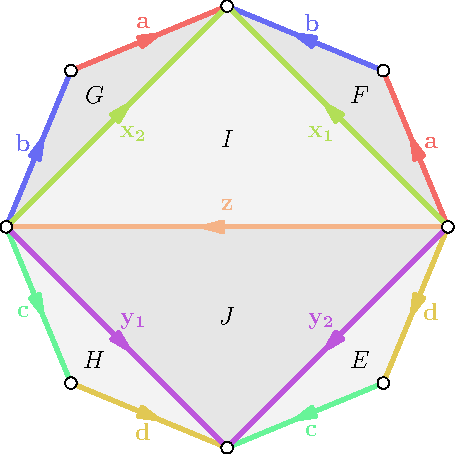
\includegraphics{C:/Users/jzchr/MathDocuments/Class Work/Topology/Homework/317Midterm/MidtermP1.pdf}
		\end{figure}
		
		The fundamental group can be derived via Van Kampen's Theorem: it is generated by the 1-simplices quotiented by the attaching maps of the 2-simplices, yielding
		$$
		\pi_1(\Sigma_2) = \frac{\<a,b,c,d,x_1,x_2,y_1,y_2,z\>}{\<bax_2^{-1},\;abx_1^{-1},\;zx_2x_1^{-1},\;cdy_1^{-1},\;dcy_2^{-1},\;zy_1y_2^{-1}\>} = \frac{\<a,b,c,d\>}{\<aba^{-1}b^{-1}cdc^{-1}d^{-1}\>}
		$$
		as $x_1=ab,\;x_2=ba,\;y_1=cd,\;y_2=dc,\;z=y_1y_2^{-1}=x_2x_1^{-1} = bab^{-1}a^{-1} = cdc^{-1}d^{-1}$.\\
		
		Now for the homology groups: there is only one 0-simplex, so $Z_0=\Z$. $B_0=0$, as the boundary of any 1-simplex is trivial, again because there is only one 0-simplex. Thus $H_0=\Z$.\\
		
		Everything in $C_1$ is a cycle because there is only one 0-simplex, so $Z_1=C_1=\Z^9$. $B_1$ is generated by the six relations given by the 2-cells:
		$$
		B_1 = \<a+b - x_1, \; b + a - x_2, \; c + d - y_1, \; d + c - y_2, \; x_1 - x_2 - z, \; y_1 - y_2 + z\>
		$$
		In the quotient $Z_1/B_1$, $x_1,x_2,y_1,y_2,z$ are all generated by $a,b,c,d$, as 
		$$x_1=x_2=a+b, \;\; y_1=y_2 = c +d, \;\; z = x_1 - x_2 = y_2 - y_1 = 0,$$
		so the homology group is just
		$$
		H_1 = Z_1/B_1 = \<a,b,c,d\> = \Z^4. 
		$$
		
		\medspace 
		
		$Z_2$ is generated by a single element. To see this, take an arbitrary element $p\in C_2$
		$$
		p := p_E\cdot E + p_F\cdot F + p_G\cdot G + p_H \cdot H + p_I \cdot I + p_J \cdot J.
		$$
		Assuming that $p\in Z_2$, we have
		\begin{align*}
		0 &= \partial p \\
		&= p_G(a + b - x_2) + p_F (a + b - x_1) + p_I (z + x_2 - x_1) + \dots\\
		&= (a+b)(p_G + p_F) + (c+d)(p_H + p_E) + x_1(p_F + p_I) + x_2(p_I - p_G) + \dots
		\end{align*}
		which implies that $p_G=p_I=p_E= -p_J=-p_H=-p_F$. Thus $Z_2$ is generated by a single element,
		$$
		Z_2 = \<E - F + G - H + I - J\>
		$$
		and $B_2$ is trivial because there are no 3-simplices. So $H_2=Z_2=\Z$.\\
		
		For any $n\geq 3$, $H_n=0$ trivially because there are no $n$-simplices in $\Sigma_2$.\\
		
		The Abelianization map $\pi_1(\Sigma_2)\to H_1(\Sigma_2)$ is just a quotient by the commutator subgroup, which is generated by $aba^{-1}b^{-1}$ and $cdc^{-1}d^{-1}$. In terms of this simplicial complex presentation, it is the quotient by $z$. Indeed, $z\equiv 0$ in $H_1(\Sigma_2)$. 
	\end{proof}\\
	
	\newpage
	\textbf{Problem 2}: Prove that $\C P^n$ does not non-trivially cover any other space.
	\begin{proof}
		$\C P^n$ can be constructed as a simplicial complex with one 0-cell $S^0$, one 2-cell $S^2$, $\dots$, and one $2n$-cell $S^{2n}$, as we've seen in class. 
%		
%		Thus, its homology is 
%		$$H_j(\C P^n) = \begin{cases}
%			\Z& j\in \{0,2,\dots,2n\}\\
%			0 & \text{otherwise}.
%		\end{cases}$$

		Suppose $p:\C P^n\to X$ is a degree $d<\infty$ covering map. Give $X$ a CW structure with one $2j$-cell $p(S^{2j})$ for $0\leq j \leq n$. None of the cells can be collapsed to a lower dimension because the degree is supposed to be finite. But then $X$ has the exact same CW structure as $\C P^n$, with the same attaching maps. Restricted to each cell, $p|_{S^{2j}}$ must be a degree-1 map because $\chi(S^{2j})=1$. So this covering can only be the identity.
	\end{proof} 
	
	\newpage
	\textbf{Problem 3}: Let $X=S^1\vee S^1$. What is $\pi_1(X)$? For each of the following covering spaces of $X$, identify the corresponding subgroup of $\pi_1(X)$ and say whether the covering is regular (i.e. normal) or not.
	
	\begin{figure}[h]
		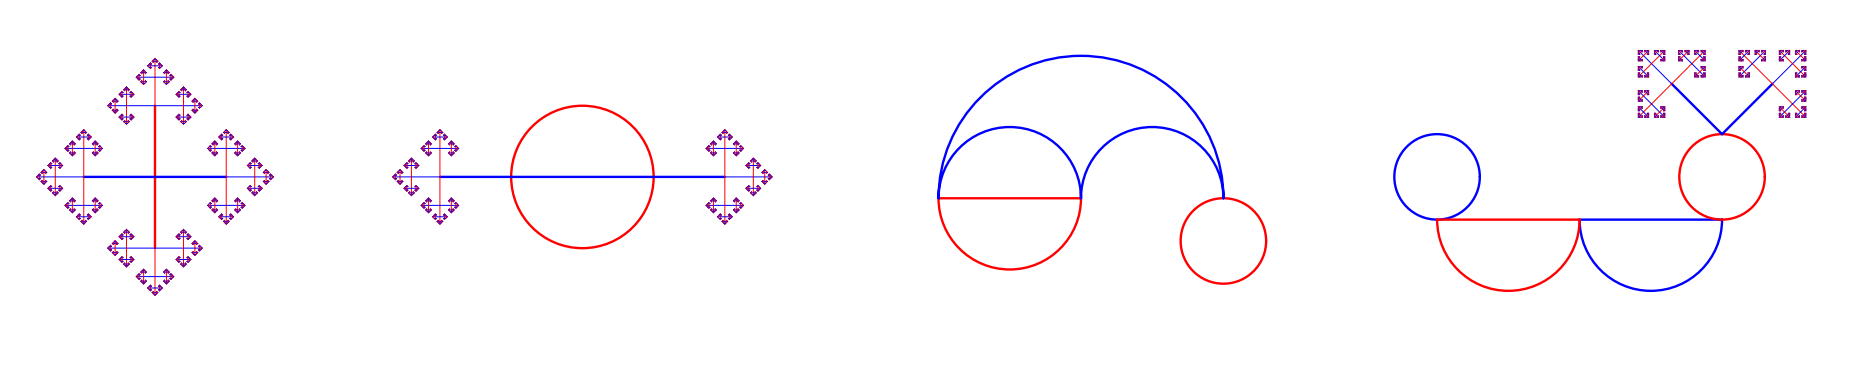
\includegraphics[width=15cm]{"C:/Users/jzchr/MathDocuments/Class Work/Topology/Homework/317Midterm/MidtermP3Fig.png"}
	\end{figure}
	
	\begin{proof}
		$\pi_1(X)$ is the free group on two generators, i.e. $\Z\ast\Z$. Let $a$ represent red and $b$ blue.\\
		
		The subgroups corresponding to each covering space can be calculated by taking representatives of edges outside a maximal spanning tree. To test whether a covering is normal, it is equivalent to test whether or not the subgroup depends on the basepoint or not (if it is the same for two given basepoints then that implies the existence of a deck transformation between them).\\
		
		(a): This is the universal cover. Its fundamental group is trivial as there are no loops. This is a regular cover because $1$ is clearly normal in $\Z\ast \Z$.\\
		
		(b): Take the basepoint to be one of the two middle points and the maximal spanning tree as all edges except the red circle. This yields the subgroup
		$$
		\<ba, \; ba^{-1}\>.
		$$
		But $ba$ is not a loop anywhere other than that basepoint, so the cover is not normal.\\
		
		(c): Take the basepoint to be the middle point among the three points and the maximal spanning tree to be the two blue edges attached to it. The resulting subgroup is
		$$
		\<ab,a^{-1}b,b^3,b^{-1}ab\>.
		$$
		The subgroup one gets from choosing the left point as the basepoint is the same, but the right point has a loop $a$ so it's not the same group. Thus, this is not a normal cover.\\
		
		(d): Take the basepoint to be the point where the two semicircles touch, and take the maximal spanning tree to be the two flat segments connected to it and one half of the red circle on the right, along with the entire free tree attached to it. This yields the subgroup
		$$
		\<aba^{-1},a^2,b^2,ba^2b^{-1}\>
		$$
		If we started from the leftmost point as the basepoint, $b$ would be in the group, but it is not, so this is also not a normal cover.
		
	\end{proof}\\
	
	\newpage
	\textbf{Problem 4}: Let $\Sigma_n$ be the closed, oriented surface of genus $n$.
	\begin{enumerate}[(a)]
		\item Show that there is a degree $p$ cover $\Sigma_m\to \Sigma_n$ iff $m=pn-p+1$.
		\item If $m=pn-p+1$, show that there is a \textit{regular} cover $\Sigma_m\to \Sigma_n$ with deck group $\Z/p\Z$. Is there more than one?
		\item In the case $n=2$ and $p=4$, compute the action of the deck group on the homology of $\Sigma_5$ for the explicit covering constructed in part (b).
	\end{enumerate}
	\begin{proof}
		(a): Suppose a degree-$p$ projection $q:\Sigma_m\to \Sigma_n$ exists. We know that such a projection multiplies the Euler characteristic by $p$. And we know that $\chi(\Sigma_g)=2-2g$. So
		$$2-2m = \chi(\Sigma_m)= p \cdot \chi(\Sigma_n) = p(2-2n) \implies m = p(n-1)+1.$$
		This proves the ``only if'' direction. For the ``if'' direction, we construct such a covering explicitly in part (b).\\

	(b): Consider the cover $\Sigma_5\to \Sigma_2$ shown below:
	
	\begin{figure}[h]
		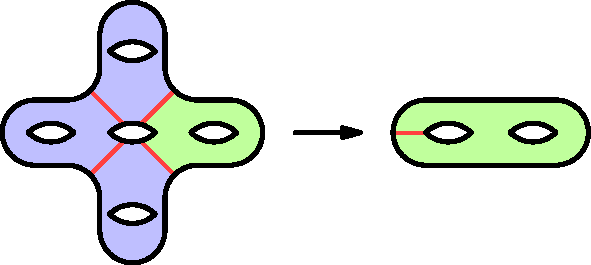
\includegraphics{C:/Users/jzchr/MathDocuments/Class Work/Topology/Homework/317Midterm/MidtermP4.pdf}
	\end{figure}
	
	The red circles are identified to close up the green sector, forming another hole. Each of the other three ``handles'' is mapped in the same way. The deck group is $\Z/4\Z$, which acts by rotating the $\Sigma_5$. Since this is transitive on the fiber of any basepoint, it is certainly a regular covering space.\\
	
%	If we present $\pi_1(\Sigma_m)$ as 
%	$$
%	\pi_1(\Sigma_m) = \Big\<a_1,b_1,a_2,b_2,\dots,a_m,b_m \; | \; \prod_j[a_j,b_j]=1\Big\> 
%	$$
%	and $\pi_1(\Sigma_n)$ as 
%	$$
%	\pi_1(\Sigma_n) = \Big\<c_1,d_1,c_2,d_2,\dots,c_{n-1},d_{n-1},x,y \; | \; \Big(\prod_j[c_j,d_j]\Big)\cdot [x,y]=1\Big\> 
%	$$
%	then $q_*$ acts as 
%	$$
%	q_*(a_{kp+j}) = x^jc_{k+1}x^{-j} , \;\;\; q_*(b_{kp+j}) = x^j d_{k+1} x^{-j}
%	$$
%	for $0\leq k\leq n-2$ and $1\leq j \leq p$, and for $a_m,b_m$,
%	$$
%	q_*(a_m) = x^{p-1}, \;\;\; q_*(b_m) = y.
%	$$
%	Note that this preserves the single relation in $\Sigma_m$:
%	\begin{align*}
%		\prod_j [q_*(a_j),q_*(b_j)] &= \Big(\prod_{k=0}^{n-2} \prod_{j=1}^p [x^jc_{k+1}x^{-j},x^{j}d_{k+1}x^{-j}] \Big)\cdot [x^{p-1},y]\\
%		&= \Big(\prod_{k=0}^{n-2} \prod_{j=1}^p x^j[c_{k+1},d_{k+1}]x^{-j}\Big)\cdot [x^{p-1},y] \\
%		&= \Big(\prod_k([c_{k+1},d_{k+1}]x)^{p-1}x^{-(p-2)} \Big)\cdot [x^{p-1},y]\\
%		&= \Big(\prod_k([c_{k+1},d_{k+1}]x)^{p-1}x^{-(p-2)} \Big)\cdot x^{p-1} (yx^{-1}y^{-1})^{p-1}\\
%		&= \Big(\prod_k([c_{k+1},d_{k+1}]x)^{p-1}x^{-(p-2)} \Big)\cdot x^{p-1} (yx^{-1}y^{-1})^{p-1}\\
%	\end{align*}\\
	
	(c): $H_0(\Sigma_5)=\Z$, as all points are equivalent mod boundaries ($\Sigma_5$ is path-connected). So $\Z/4\Z$ acts trivially on $H_0(\Sigma_5)$.
	
	$H_1(\Sigma_5)=\Z^{10}$, generated by two loops for each hole. If these loops are $\<a_1,b_1,\dots,a_5,b_5\>$ then $\Z/4\Z$ acts on these by rotating the outer loops and fixing the inner one.
	
	$H_2(\Sigma_5)=\Z$, generated by the single 2-cell (or a linear combination of all 2-simplices). $\Z/4\Z$ acts trivially.
	
	\end{proof}
	 
	 \newpage
	 \textbf{Problem 5}: Show that the universal cover of the Klein bottle is homeomorphic to a plane. Deduce that the Klein bottle is a $K(\pi,1)$ and conclude that its fundamental group is torsion-free.
	 
	 \begin{proof}
	 	$\R^2$ covers the Klein bottle via the covering map depicted below:
	 	
	 	\begin{figure}[h]
	 		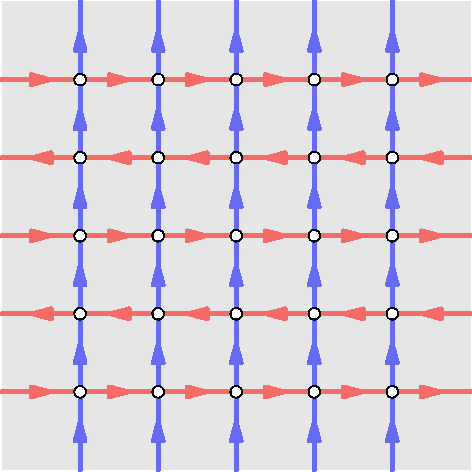
\includegraphics{C:/Users/jzchr/MathDocuments/Class Work/Topology/Homework/317Midterm/MidtermP5.pdf}
	 	\end{figure}
	 	
	 	The plane is clearly contractible, so this is the universal cover and the Klein bottle is a $K(\pi,1)$.\\
	 	
	 	As we showed in class, if a $K(\pi,1)$ has finite dimension then $\pi$ is torsion-free. It follows that the Klein bottle's fundamental group is torsion-free as well.
	 	
	 	Alternatively, one could explicitly state the multiplication rules for $\pi$ and see that it is torsion-free. We have
	 	$$
	 	\pi := \<a,b\; | \; ab=ba^{-1}\>
	 	$$
	 	so every element in $\pi$ can be written uniquely as $a^nb^m$ for some $n,m\in \Z$, with multiplication given by 
	 	$$
	 	(a^nb^m)\cdot (a^pb^q) = \begin{cases}
	 		a^{n-p}b^{m+q} & m \text{ is odd}\\
	 		a^{n+p}b^{m+q} & m \text{ is even}
	 	\end{cases}
	 	$$
	 	so as one can see, powers of any element $a^nb^m$ with $m\neq 0$ can never be 1, and clearly powers of $a^n$ can never be 1 either.
	 \end{proof}
	 
	 \newpage 
	 \textbf{Problem 6}: The figure 8 knot is the embedded circle in the 3-sphere shown in the figure below. Compute the fundamental group and the homology groups of the complement of the knot in $S^3$.
	 \begin{figure}[h]
	 	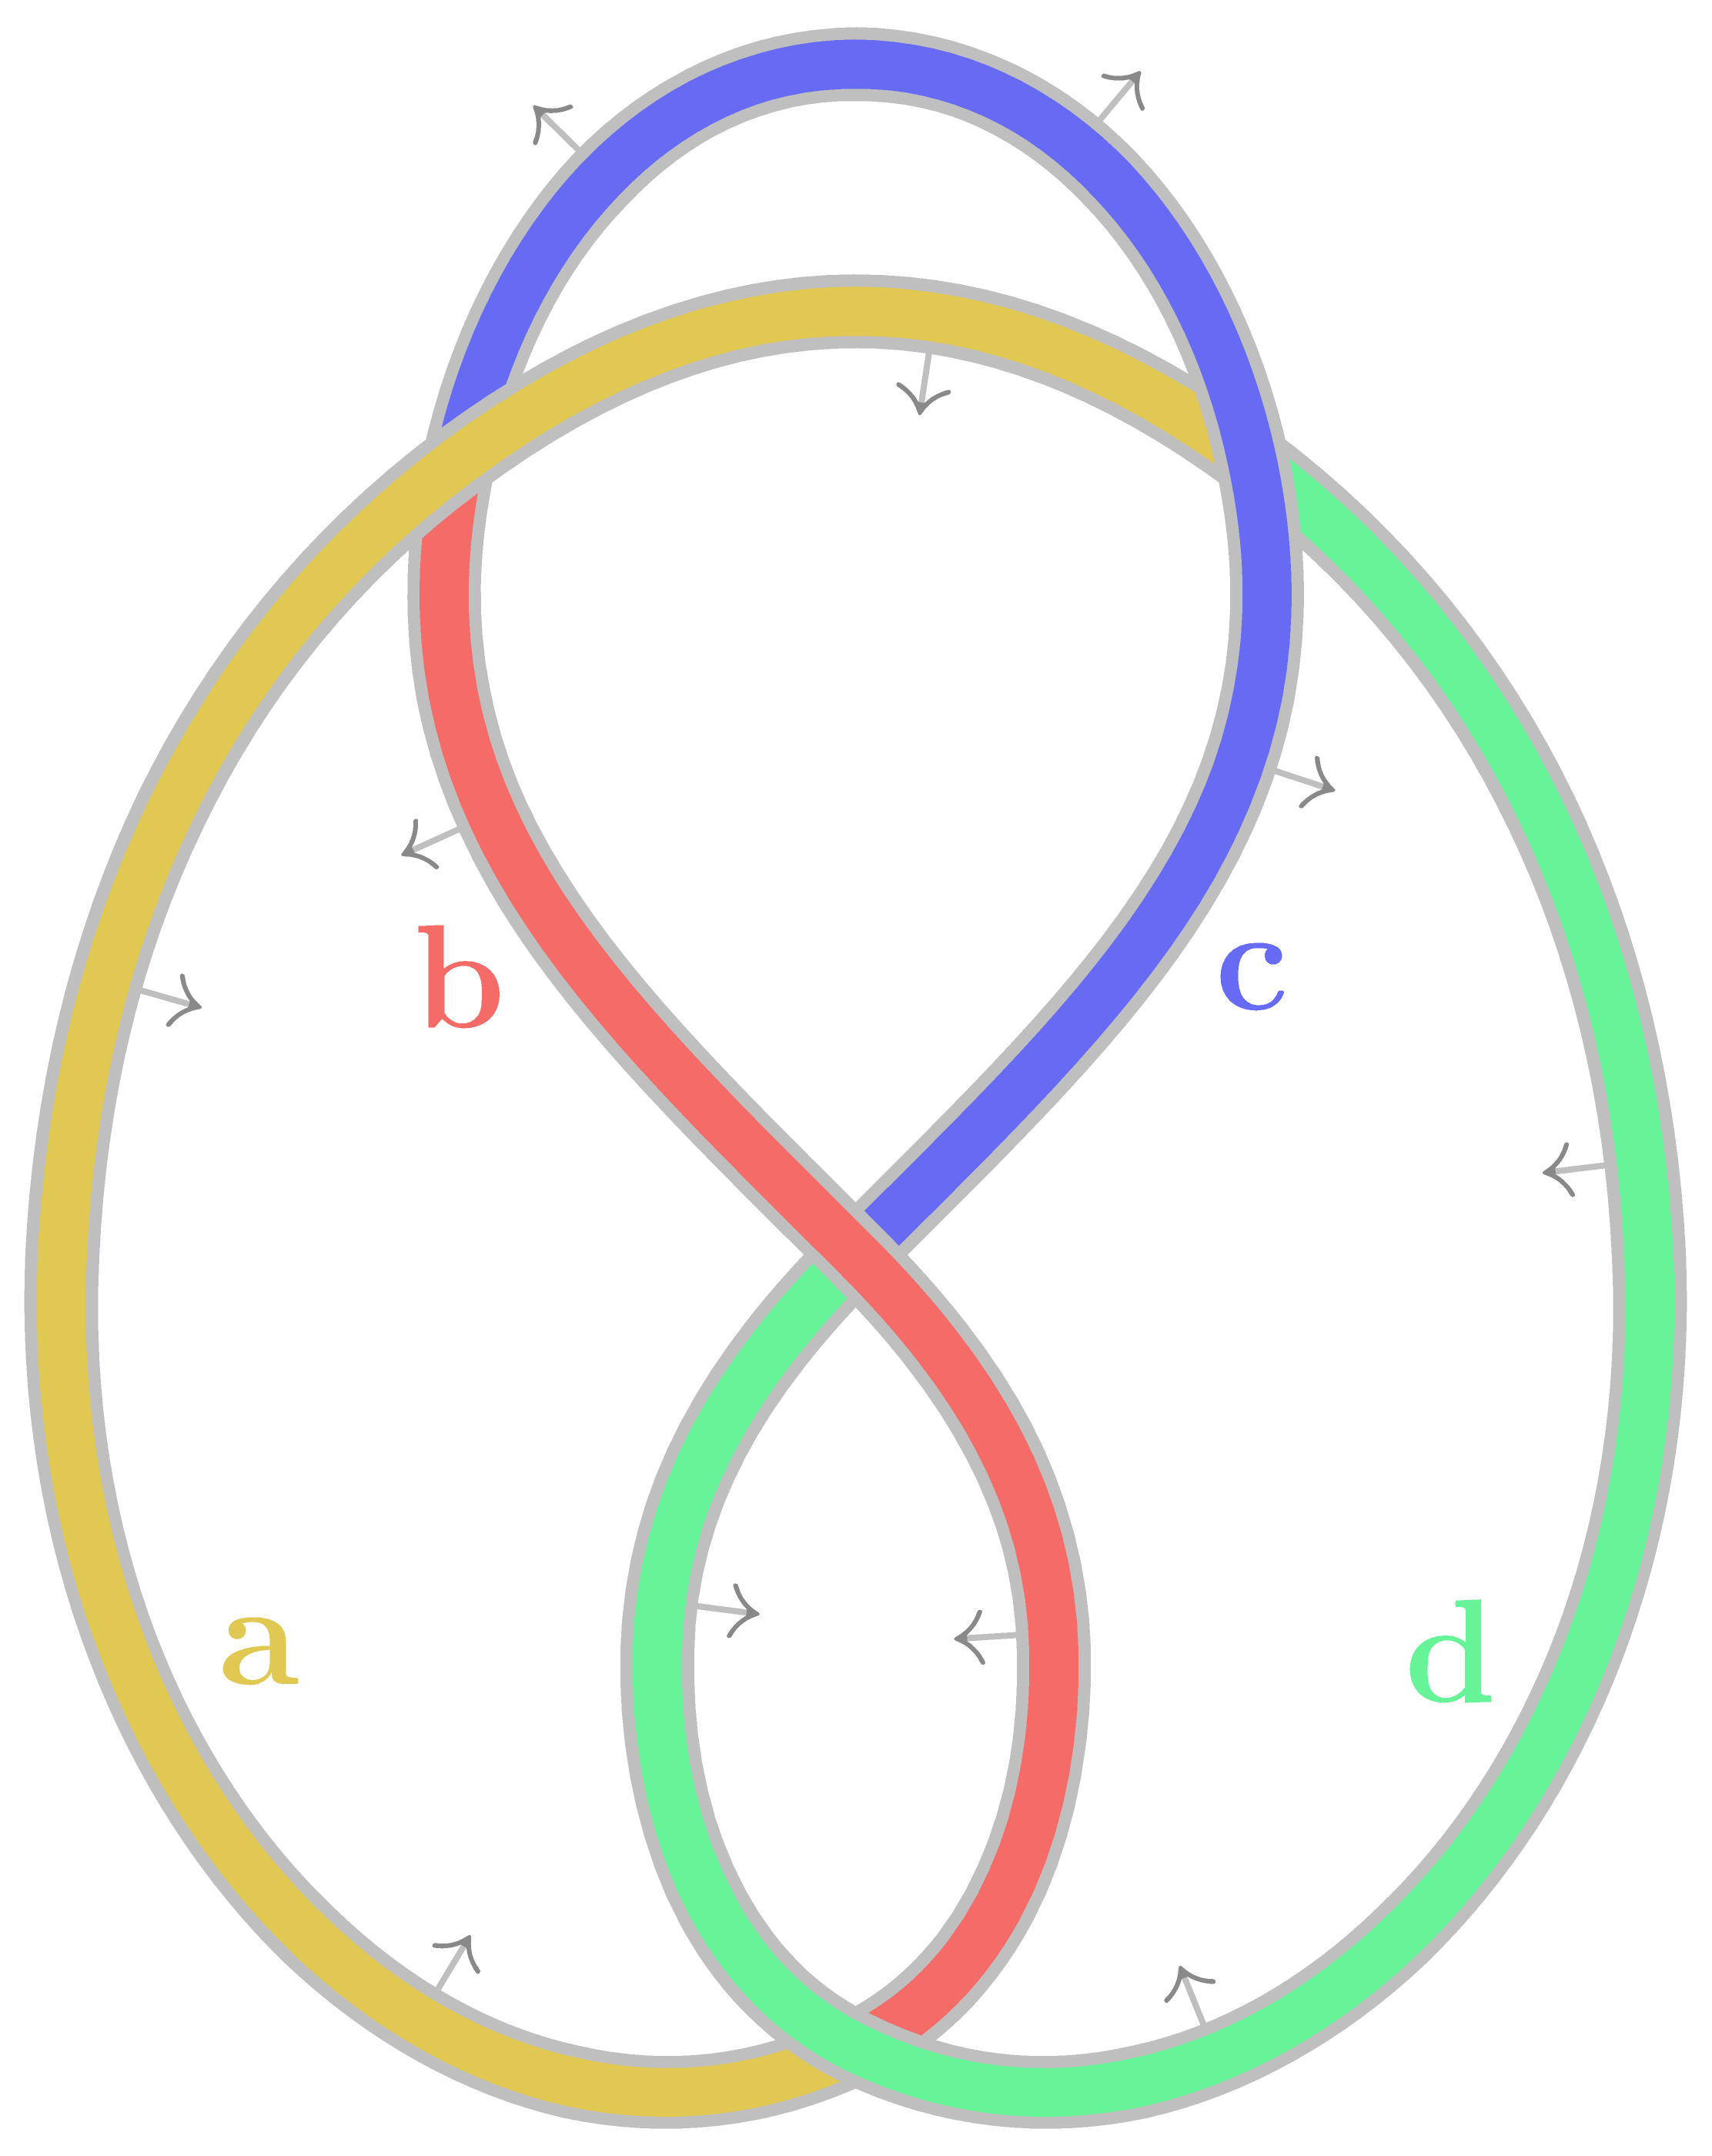
\includegraphics[width=6cm]{"C:/Users/jzchr/MathDocuments/Class Work/Topology/Homework/317Midterm/MidtermP6.png"}
	 \end{figure}
	 
	 Let this knot be $K\subset S^3$, with the orientation indicated by the arrows. We can use the Wirtinger presentation of $\pi_1(S^3\setminus K)$ as described in a homework problem. It is generated by four elements $a,b,c,d$ corresponding to unbroken knot-segments when viewed from below, which denote 1-cells crossing those segments in the direction given by the knot's orientation (here I've depicted the knot from above, though it shouldn't affect the fundamental group). The relations between $a,b,c,d$ are given by conjugation at the crossing-points:
	 \begin{align*}
	 \pi_1(S^3\setminus K) &= \<a,b,c,d \; | \; aba^{-1}=c, \;\; dbd^{-1} = a, \;\; cdc^{-1} = a, \;\; bdb^{-1} = c\>\\
	 &= \<b,d \; | \; bdb^{-1}dbd^{-1}b^{-1}db^{-1}d^{-1} = 1\>
	 \end{align*}
	 In the Abelianization of this group, this becomes $\<b,d \; | \; b^{-1}d=1\>=\Z$. Thus, $H_1(S^3\setminus K)=\Z$.\\
	 
	 To compute the other homology groups, note that (as described in this same recent homework problem) $S^3\setminus K$ can be deformation retracted to a 2-dimensional CW complex $X$ (or a 2-dimensional simplicial complex). Thus, the homology groups of $S^3\setminus K$ are the same as those of $X$. 
	 
	 $H_0(S^3\setminus K)=\Z$, as $X$ is connected, so every $0$-cell is identified when taking the quotient by boundaries. 
	 
	 $H_1(S^3\setminus K)=\Z$ as already shown above. 
	 
	 $H_2(S^3\setminus K)=Z_2(X)$, as $B_2(X)$ is trivial (there are no 3-simplices in $X$ hence no 2-boundaries). When $X$ is constructed as a CW complex, the 2-cells (corresponding to the squares covering crossings) have boundaries 
	 $$
	 a + b - a - c, \; d + b - d - a, \; c + d - c - a,\; b + d - b - c.
	 $$
	 If the coefficients of these in some 2-cycle $p$ are $p_1,p_2,p_3,p_4$, then 
	 $$
	 \partial p = p_1(b-c) + p_2(b-a) + p_3(d-a) + p_4(d-c) = a(-p_2-p_3) + b(p_2+p_1) + c(-p_1-p_4) + d(p_3+p_4).
	 $$
	 If $p$ is a cycle, then $\partial p =0$, so 
	 $$
	 p_1 = -p_2 = p_3 = -p_4
	 $$
	 so $Z_2(X)$ is spanned by a single 2-cycle with coefficients in this proportion. Thus $H_2(S^3\setminus K)=\Z$.
	 
	 
%	 We will now show $H_2(S^3\setminus K)=0$. Let $C$ be a solid open tube surrounding $K$ which does not intersect itself, so that $C$ is homeomorphic to $S^1\times D$ and homotopy-equivalent to $S^1$. The Mayer-Vietoris sequence gives
%	 $$
%	 \cdots \to H_3(X)\oplus H_3(C) \to H_3(S^3) \to H_2(X\cap C)\to H_2(X)\oplus H_2(C) \to H_2(S^3)\to \cdots
%	 $$
%	 We determine all of these groups but $H_2(X)$ as follows. Since $C$ is deformation-retractable to $S^1$, $$H_3(C)=0, \; H_2(C)=0, \; H_1(C)=\Z, \; H_0(C)=\Z.$$ 
%	 Moreover, $X\cap C$ is deformation-retractable to the hollow torus $S^1\times S^1$. This gives
%	 $$
%	 H_3(X\cap C) = 0, \; H_2(X\cap C) = \Z, \; H_1(X\cap C) = \Z^2, \; H_0(X\cap C) = \Z.
%	 $$ 
%	 And we also know that $H_3(X)=0$ because $X$ has no 3-cells and $H_n(S^3)=\Z$ iff $n=3$, and 0 otherwise. With this information, the sequence becomes
%	 $$
%	 \cdots \to 0 \to \Z \to \Z \to H_2(X)\oplus 0 \to 0\to \cdots
%	 $$
%	 The sequence is exact, so $H_2(X)$ is some quotient of $\Z$, depending on the scale factor of the map $H_3(S^3)\to H_2(X\cap C)$. And what is this scale factor?\\
	 
	 $H_n(S^3\setminus K)=0$ for $n\geq 3$, as there are no $3$-cells in $X$.
	 
	 \newpage
	 \textbf{Problem 7}: State and prove the Five Lemma.
	 
	 \begin{proof}
	 	Given an exact sequence of five Abelian groups $A,B,C,D,E$ with group homomorphisms $p_{\bullet}$ to another exact sequence $A',B',C',D',E'$ such that the below diagram commutes, we would like to show that if $p_A,p_B,p_D,p_E$ are isomorphisms, then $p_C$ is as well.
	 $$
	 \begin{tikzcd}
	 	A && B && C && D && E \\
	 	\\
	 	{A'} && {B'} && {C'} && {D'} && {E'}
	 	\arrow["{f_1}", from=1-1, to=1-3]
	 	\arrow["{p_A}"', tail reversed, from=1-1, to=3-1]
	 	\arrow["{f_2}", from=1-3, to=1-5]
	 	\arrow["{p_B}"', tail reversed, from=1-3, to=3-3]
	 	\arrow["{f_3}", from=1-5, to=1-7]
	 	\arrow["{p_C}"{description}, from=1-5, to=3-5]
	 	\arrow["{f_4}", from=1-7, to=1-9]
	 	\arrow["{p_D}", tail reversed, from=1-7, to=3-7]
	 	\arrow["{p_E}", tail reversed, from=1-9, to=3-9]
	 	\arrow["{g_1}"', from=3-1, to=3-3]
	 	\arrow["{g_2}"', from=3-3, to=3-5]
	 	\arrow["{g_3}"', from=3-5, to=3-7]
	 	\arrow["{g_4}"', from=3-7, to=3-9]
	 \end{tikzcd}
	 $$
%	 To do this we will use the following useful fact about commutative squares with isomorphisms: if one has the following commutative diagram
%	 $$
%	 \begin{tikzcd}
%	 	A && B \\
%	 	\\
%	 	{A'} && {B'}
%	 	\arrow["{f_1}", from=1-1, to=1-3]
%	 	\arrow["{p_A}"', tail reversed, from=1-1, to=3-1]
%	 	\arrow["{p_B}"', tail reversed, from=1-3, to=3-3]
%	 	\arrow["{g_1}"', from=3-1, to=3-3]
%	 \end{tikzcd}
%	 $$
%	 then $a\in \ker(f_1)$ iff $p_A(a)\in \ker(g_1)$, and $b\in \im(f_1)$ iff $p_B(b)\in \im(g_1)$. This is easy to show, as $g_1(p_A(a)) = p_B(f_1(a)) = p_B(0) = 0$.\\
	 
	 We'll construct the inverse of $p_C$. Given $y\in C'$, we have $g_3(y)\in D'$ and $z := p_D^{-1}(g_3(y))\in D$. By exactness of the bottom sequence, $g_3(y)\in \ker(g_4)$, so by the commutativity of the rightmost square, 
	 $$f_4(z) \in \ker(p_E) \implies f_4(z) = 0 \implies z\in \im(f_3)$$
	 using the fact that $p_E$ is an isomorphism. So take some $x\in C$ such that $f_3(x)=z$. It is clear by the commutativity of the $C,D,C',D'$ square that $p_C(x)=y$. Now it remains to show that this $x$ is unique. 
	 
	 It suffices to show that if $p_C(x)=0$ then $x=0$, since if $p_C(x)=p_C(x')$ then 
	 $$
	 p_C(x) - p_C(x') = p_C(x-x') = 0 \implies x=x'.
	 $$
	 So suppose $p_C(x)=0$. Then $f_3(x)=0$ because $p_D$ is an isomorphism, so $x\in \im(f_2)$. Let $w\in B$ such that $f_2(w)=x$. Again by commutativity, $g_2(p_B(w))=0$, so $p_B(w)\in \im(g_1)$, and thus because $p_A$ is an isomorphism $w\in \im(f_1)$. But this implies that $w\in \ker(f_2)$, so $0=f_2(w)=x$.
	 
	 \end{proof}
\end{document}





















